\documentclass[paper=a4, fontsize=11pt]{scrreprt}

\usepackage[utf8]{inputenc}
\usepackage[ngerman,english]{babel}
\usepackage{gensymb}

\usepackage[yyyymmdd]{datetime}
\renewcommand{\dateseparator}{-}

\usepackage{hyperref}

\usepackage{tikz}
\usetikzlibrary{arrows}
\usetikzlibrary{decorations.pathreplacing}

\usepackage{natbib}
\bibliographystyle{plain}

\usepackage{minted}
%\usemintedstyle{rainbow_dash}

\usepackage{amsmath}
\usepackage{mathtools}

\usepackage{wrapfig}
\usepackage{multicol}
\usepackage{color}
\usepackage{pifont}

\title{Autonomous Parking Scenario}
\subtitle{Linux and L4, SS 2017, Group 03}
\author{Alexander Reisner \href{mailto:reisner@tum.de}{\texttt{reisner@tum.de}} \and
Alexander Weidinger \href{mailto:alexander.weidinger@tum.de}{\texttt{alexander.weidinger@tum.de}} \and
David Werner \href{mailto:david.werner@tum.de}{\texttt{david.werner@tum.de}}}
\date{\today}

\begin{document}

% title page
\maketitle
\newpage

% toc
\tableofcontents
\newpage

% introduction
\chapter{Introduction (Alexander Weidinger)}
This document is the final report, written by the students Alexander Reisner,
Alexander Weidinger and David Werner, for the "Linux and L4" SS 2017 practical course at the Technical University of Munich.

The overall given task for the practical course was to implement an autonomous parking algorithm.

This parking algorithm is implemented as an user space application for a Pandaboard,
running the Genode OS Framework in version 16.08 with the Fiasco.OC version r56 as kernel.
We will refer to this compound as \textit{ECU} from now on.

Our ECU is integrated in the hybrid simulator framework preexisting by the KIA4SM project.
This hybrid simulator consists of a car racing simulator, Speed Dreams 2 (SD2),
a simulation coupler (SimCoupler), a so called \textit{S/A VM} which basically represents a multiplexing entity for each car in the simulation
and a model car, representing the main car in the simulation.

Operating the model car is not part of this group's task but rather a task of the second team in this practical course.
Due to the structure of the data exchange that was agreed on at the Level of the ECU and S/A VM,
calculated actuator data is also received by the other team's software and can be used to control the model car.

\section{Project Overview}
Figure \ref{aw_overview} shows the overview of the project
and the information flow between all involved components.
SD2 produces sensor information and sends them to the S/A VM.
The S/A VM multiplexes the data and publishes all information to the ECUs.
They are now able to compute control commands and publish them back to the S/A VM.
The S/A VM now itself receives all control commands, bundles them in a single messages
and sends them back to SD2.
This behavior runs endlessly in a loop and gets executed each simulation step.

\begin{figure}[H]
  \begin{center}
    \begin{tikzpicture}[scale=1]
      \node[draw] at (5,0) (a){SD 2};
      \node[draw] at (5,-4) (c){S/A VM};
      \node[draw] at (0, -4) (d){ECU};
      \draw[->] (a) -- node[right] {\textit{\tiny Send sensor data}} (c);
      \draw[->, transform canvas={xshift=-0.15cm}] (c) -- node[left] {\textit{\tiny Forward actuator data}} (a);
      \draw[->, transform canvas={yshift=0.15cm}] (c) -- node[above] {\textit{\tiny Forward sensor data}} (d);
      \draw[->, transform canvas={yshift=-0.15cm}] (d) -- node[below] {\textit{\tiny Receive actuator data}} (c);
      \draw[->] (d) to [out=180,in=270,looseness=8] node [above left,xshift=-0.25cm,align=right]{\tiny\textit{Calculate next step}\\ \tiny\textit{in parking algorithm}} (d);
    \end{tikzpicture}
  \end{center}
  \caption{Overview of components}\label{aw_overview}
\end{figure}

\section{Sub Tasks}
The project was split into sub tasks, assigned to each member of the group
and also represents the parts written by each one in this report:

\begin{itemize}
  \item \textbf{Alexander Reisner}
  \begin{itemize}
    \item Design and Implementation of the S/A VM
    \item Data exchange between S/A VM and SD2
    \item Data exchange between S/A VM and ECU
    \item Implementation of the connection interface (Mosquitto client) in the ECU
    \item Final port of the Mosquitto library to the Genode OS Framework
  \end{itemize}
  \item \textbf{Alexander Weidinger}
  \begin{itemize}
    \item Extension of SD2 by a proximity sensor
    \item Data exchange between SD2 and S/A VM
    \item Extension of the human driver bot to enable autonomous driving
    \item Extend SD2 by a parked car driver bot
    \item Change starting grid of cars to allow reproducible testing results
  \end{itemize}
  \item \textbf{David Werner}
  \begin{itemize}
    \item Implement the autonomous parking algorithm
    \item Optimize the algorithm and adapt it for usage in our scenario
  \end{itemize}
\end{itemize}

% -------------------------
% changes to speed dreams 2
% -------------------------
\chapter{Speed Dreams 2 (Alexander Weidinger)}
Speed Dreams 2 is a fork of The Open Racing Car Simulator (TORCS)
and was used as our main car simulation.
Since the simulator was merely intended as a racing simulator,
it only provides limited functionality in case of (virtual) sensors.
Fortunately it can be easily expanded since the project itself is open source
and more or less sufficiently documented for such tasks.
Additionally there is a mailing list\footnote{\url{https://sourceforge.net/p/speed-dreams/mailman/}}
and an online forum\footnote{\url{https://community.speed-dreams.org/}},
where other people are willing to help in case of questions.

For our autonomous parking use case we needed to make some changes to SD2,
which affect the proximity sensor itself, the starting position of the cars
and finally changes to the driving bots.

% proximity sensor
\section{Proximity Sensor}
Since SD2 itself doesn't provide virtual proximity sensors,
we either need to implement one ourselves or we make use of related projects.
Luckily there exists the "Simulated Car Racing Championship 2015" (SCRC) \cite{scrc2015},
which extends the TORCS simulator by two new sensors.
One being an "opponent" sensor, which measures the distance between the driving car and an opponent,
furthermore there is a "focus" sensor, which measures the distance between the car and the track edge.

% reference implementation by the SCRC
\subsection{SCRC Implementation}
The problem with the given implementation is,
that the opponent sensor just measures the distance between two cars given the middle point of both cars.
Given the example in figure \ref{aw_scrc_impl}, the distance between both cars should be relatively small,
since they are more or less next to each other.
But due to the implementation, the distance $d_1$ is over 2 meters and if they were directly next to each other,
the distance between both cars would still be exactly 2 meters (given that each car has a width of 2 meters).
Therefore the distance given by this sensor can be used to get a basic idea on where other cars are
and how far they are away from oneself but are completely useless for our parking scenario.
The red dashed lines in the figure additionally shows the way how distances to objects are sorted into multiple proximity "sensors",
by calculating the angle between both cars and mapping it into a sensor.
The implementation gives a 360\degree{} view by splitting it in intervals of 30\degree{}\footnote{Different values for the interval is also possible.}.

\begin{figure}
\begin{center}
\begin{tikzpicture}[scale=1]
  % car 1
  \draw (0,0) -- (2,0) -- (2,3) -- (0,3) -- (0,0);
  \fill (1, 1.5) circle [radius=0.05];
  % car 2
  \draw (3,1) -- (5,1) -- (5,4) -- (3,4) -- (3,1);
  \fill (4, 2.5) circle [radius=0.05];
  % line between the two midpoints
  \draw (1, 1.5) -- (4, 2.5);
  % sensor lines
  \foreach \x in {0, 30, ..., 330} \draw[red, dashed] (1, 1.5) -- +(\x : 3);
  % distance bracket
  \draw[decoration={brace,mirror,raise=5pt},decorate] (1, 1.5) -- (4, 2.5) node[black,midway,yshift=-0.5cm] {\footnotesize $d_1$};
\end{tikzpicture}
\end{center}
\caption{Proximity sensor implemented by the Simulated Car Racing Championship 2015}\label{aw_scrc_impl}
\end{figure}

% our own implementation
\subsection{Our Implementation}
\subsubsection{Idea}
We simplify the virtual proximity sensor to a mere straight line,
with a given angle and position relative to the center of the car.

The opponent car can be cut down to four straight lines,
acting as the four sides of a car.

In order to now calculate the shortest distance to an opponent car,
the algorithm takes the following steps:

\begin{enumerate}
  \item Iterate over all opponent cars:
  \begin{enumerate}
    \item Calculate intersections between the straight line from the laser
    and the four straight lines from the sides of the opponent car.
    \item Iterate over all intersections:
    \begin{enumerate}
      \item Test if point of intersection is within the domain of the respective side of the car.
      \item\label{infront} Check if the intersection is "in front" of the sensor.
    \end{enumerate}
    \item Save the potentially shortest distance to an opponent, if not already a shorter distance was found.
  \end{enumerate}
  \item Accept the shortest distance as the current value of the proximity sensor.
\end{enumerate}

Step \ref{infront} is necessary, since we are working with straight lines
and not vectors. Otherwise it could happen,
that objects on the other side of the car have to shortest distance to the sensor
and therefore are accepted incorrectly as the current value of the sensor.
A mockup of our implementation idea can be seen in figure \ref{aw_mockup}.
The distance $d_2$ would be the correct value for the proximity sensor,
indicated by the dashed blue line.

\begin{figure}[ht]
  \begin{center}
    \begin{tikzpicture}[scale=1]
      % car 1
      \draw (0,0) -- (2,0) -- (2,3) -- (0,3) -- (0,0);
      \fill (1, 1.5) circle [radius=0.05];
      % car 2
      \draw (3,1) -- (5,1) -- (5,4) -- (3,4) -- (3,1);
      \fill (4, 2.5) circle [radius=0.05];
      % sensor
      \draw[blue, dashed] (2, 1.5) -- +(0 : 4); % line
      \fill[blue] (2, 1.5) circle [radius=0.05]; % starting point
      % intersections
      \draw[blue] (3, 1.5) circle [radius=0.1];
      \draw[blue]  (5, 1.5) circle [radius=0.1];
      % distance bracket
      \draw[decoration={brace,mirror,raise=5pt},decorate] (2, 1.5) -- (3, 1.5) node[black,midway,yshift=-0.5cm] {\footnotesize $d_2$};
    \end{tikzpicture}
    \caption{Mockup of our (laser) proximity sensor implementation}\label{aw_mockup}
  \end{center}
\end{figure}

\subsubsection{Implementation}
Since a sensor position is described as a relative point to the center $(0,0)$ of a car,
we need to move the starting point of the sensor to the correct absolute position.
The distance from the center point to the sensor is calculated
and the x and y coordinates are added to the absolute position of the car,
in regard to the yaw of the car (see listing \ref{aw_sensor_position}).

\begin{listing}[ht]
  \inputminted[firstline=91,linenos=true,lastline=96,gobble=2]{c++}{../../../simulators/speed-dreams/src/libs/sensors/obstacleSensors.cpp}
  \caption{\texttt{src/libs/sensors/obstacleSensors.cpp}}\label{aw_sensor_position}
\end{listing}

To calculate the straigt line equation $m*x+t=y$ of the sensor,
$m$ must be calculated by adding the custom angle to the current yaw of the car using $tan$.
$t$ can be then obtained by simple inserting the $x$ and $y$ coordinates of the sensor.
The associated code can be seen in listing \ref{aw_mt}.

\begin{listing}[ht]
  \inputminted[firstline=105,linenos=true,lastline=104,gobble=2]{c++}{../../../simulators/speed-dreams/src/libs/sensors/obstacleSensors.cpp}
  \vspace{-0.3cm}...\vspace{-0.3cm}
  \inputminted[firstline=110,linenos=true,lastline=109,gobble=2]{c++}{../../../simulators/speed-dreams/src/libs/sensors/obstacleSensors.cpp}
  \caption{\texttt{src/libs/sensors/obstacleSensors.cpp}}\label{aw_mt}
\end{listing}

After calculating the straight line equation for the sensor,
we need to create four additional ones, representing the four sides of the car.
We calculate the slope $m$ by using the yaw of the car, to get the left and right sides.
For the front and back sides we do the same but use the yaw $+$90\degree{} for the rotation.
These four straight lines are moved to the correct position,
again relative to the center of the obstacle car (compare listing \ref{aw_mt_obst}).

\begin{listing}[ht]
  \inputminted[firstline=130,linenos=true,lastline=152,gobble=3]{c++}{../../../simulators/speed-dreams/src/libs/sensors/obstacleSensors.cpp}
  \caption{\texttt{src/libs/sensors/obstacleSensors.cpp}}\label{aw_mt_obst}
\end{listing}

Now that all five straight lines are calculated,
the next step is the computation of the intersections between the straight line of the sensor
and the four straight lines, representing the sides of the obstacle car (see listing \ref{aw_intersect}).

\begin{listing}[ht]
  \inputminted[firstline=154,linenos=true,lastline=164,gobble=3]{c++}{../../../simulators/speed-dreams/src/libs/sensors/obstacleSensors.cpp}
  \caption{\texttt{src/libs/sensors/obstacleSensors.cpp}}\label{aw_intersect}
\end{listing}

After obtaining the intersections, the domain is checked by verifying,
that the intersection is between the two points restricting the side of the car.
Additional to that, we need to make sure the obstacle isn't behind the sensor.
For that we reuse our \texttt{is\_between} function (which checks if a point is between two points) and adding a reference point,
which basically is just an additional point "behind" the sensor in a fixed distance (see listing \ref{aw_ref}).

\begin{listing}[ht]
  \inputminted[firstline=98,linenos=true,lastline=99,gobble=2]{c++}{../../../simulators/speed-dreams/src/libs/sensors/obstacleSensors.cpp}
  \caption{\texttt{src/libs/sensors/obstacleSensors.cpp}}\label{aw_ref}
\end{listing}

Now that we can find the intersections between a sensor and an obstacle car,
we do this in a loop for all sensors and all cars.
That way we can determine the shortest distance overall for each sensor
and set it as the correct distance value for the respective sensor.

\subsubsection{Usage}
As an example on how to use the newly created obstacleSensors library,
one can take a look at the human driver in listing \ref{aw_sensors}.

\begin{listing}[ht]
  \inputminted[firstline=245,linenos=true,lastline=256,gobble=4]{c++}{../../../simulators/speed-dreams/src/drivers/human/human.cpp}
  \caption{\texttt{src/drivers/human/human.cpp}}\label{aw_sensors}
\end{listing}

The code adds three sensors, one in the front with an 0\degree{} angle
and one in the back with an angle of 180\degree{}.
Both sensors are moved relative to the center point of the car,
according to the schematics in the comment.
The last sensor (second sensor in the example code) is directed in an 90\degree{} angle
and moved to the right side of the rear axle.
As a side note, all three sensors have a maximum range of 20 meters,
which can be changed with the last parameter.

\subsubsection{Evaluation}
\begin{figure}[ht]
  \begin{center}
  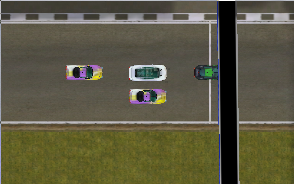
\includegraphics[scale=0.5]{aw_imgs/parked.png}
\end{center}
\caption{test}\label{aw_parked_img}
\end{figure}

Given the situation in figure \ref{aw_parked_img}
(we are the white car) and having one sensor in the front,
one in the back and one to the right,
we receive the following values for the sensors:
\begin{itemize}
  \item \textbf{Front:} 3.306382 m
  \item \textbf{Back:} 3.400575 m
  \item \textbf{Right:} 1.010126 m
\end{itemize}

While with the implementation by the SCRC project,
we receive different values:
\begin{itemize}
  \item \textbf{Front:} 8.086382 m
  \item \textbf{Back:} 8.180575 m
  \item \textbf{Right:} 3.010126 m
\end{itemize}

This means, that our sensor implementation is much more precise
and usable for the parking scenario.

\subsubsection{Open points}
Our main focus was getting the overall setup running,
therefore a few open points are still left open
and can be fixed in future versions.

The whole implementation is based on straight lines
and therefore needs some workarounds to deal with directions.
To overcome this issue it would make sense to change the implementation to vectors.
This could also fix some potential glitches with wrong distance values,
which can occur on collisions due to precision errors.
Lastly the implementation only represents a laser proximity sensor
in contrast to the implementation by the SCRC,
which can detect or more precisely assigns opponents in angle ranges.
One could work around this limitation by randomizing the direction of the laser sensor in a specific range of angles
and afterwards taking the average of these values.

\section{Starting Grid}
In order to test the successful execution of our parking algorithm,
we need to be able to get reproducible results in every run.

\subsection{Idea}
As we are not able to create some kind of run configuration files for SD2
and an implementation of such a system would take a lot of work,
we made use of the starting grid in the initialization phase of a race.

\subsection{Implementation}
Normally the \textit{*.xml} file of a SD2 track specifies the number of rows,
the cars are placed in at the start line.
The distance between the cars is then automatically adjusted and calculated,
taking in mind the overall width of the track, the course of the road, etc.

For the purpose of the parking scenario we hard coded the row value to one,
as can be seen in listing \ref{aw_rows}.
\begin{listing}[ht]
  \inputminted[firstline=309,linenos=true,lastline=311,gobble=1]{c++}{../../../simulators/speed-dreams/src/modules/racing/standardgame/raceinit.cpp}
  \caption{\texttt{src/modules/racing/standardgame/raceinit.cpp}}\label{aw_rows}
\end{listing}

We also made sure to place each car 8 meters further away from the start line by choosing a fix value in the code.
Additionally to get the second and last car to either be 3 meters to the left or right,
we adapted the position change to the right accordingly in the code (listing \ref{aw_dist}).
\begin{listing}[ht]
  \inputminted[firstline=316,linenos=true,lastline=327,gobble=4]{c++}{../../../simulators/speed-dreams/src/modules/racing/standardgame/raceinit.cpp}
  \caption{\texttt{src/modules/racing/standardgame/raceinit.cpp}}\label{aw_dist}
\end{listing}

In order to ensure, that the changes don't interfere with future development,
the changes only get used, if the code is compiled with the \texttt{PARKING} option enabled.

\section{Driving bots}
Further changes were needed for two of the bots in SD2,
since we still want to be able to drive for ourselves,
although we need to make sure that the car can move autonomously.
Additionally we need parked cars for our proximity sensor to detect.
We chose to make use of the \textit{human} driver for the first use case
and extend it by the autonomous driving.
For the second use case we chose the \textit{usr} driver to act as the parked car.

\subsection{human}
The changes to the \textit{human} bot consists of two parts.
First add the data exchange between SD2 and the S/A VM
and second include an autonomous driving logic.

The code for the data exchange is relatively trivial,
since its a simple socket based connection,
where SD2 acts as the server and globally listens for connections on port 9002\footnote{The listen address and port can be changed at the top of the \texttt{human.cpp} file}.
The only really relevant part is, that one needs to disable Nagle's algorithm,
by setting the \texttt{TCP\_NODELAY} socket option,
because we are creating a real time application and are in need of a low latency.\footnote{A short explanation of Nagle's algorithm can be found in section \ref{ar_naglealgo}.}
The message flow between the S/A VM and SD2 is always the same
and based on an exchange between both applications.
First SD2 collects all sensor information (proximity sensors, spin velocity of the wheels, etc.)
and packs this data into a Protobuf \textit{State} message.\footnote{For an explanation of the Google Protobuf protocol see section \ref{ar_protobuf_subsection}.}

The Protobuf message is then serialized to a string,
the length of this message gets extracted
and both information are transmitted over the socket connection,
as can be seen in listing \ref{aw_send}.

\begin{listing}[ht]
  \inputminted[firstline=352,linenos=true,lastline=363,gobble=4]{c++}{../../../simulators/speed-dreams/src/drivers/human/human.cpp}
  \caption{\texttt{src/drivers/human/human.cpp}}\label{aw_send}
\end{listing}

For the back channel, SD2 receives a Protobuf \textit{Control} message from the S/A VM,
following the same protocol (message length, message content).
This message is parsed and information about the desired speed,
the intended steering angle
and if the car will drive autonomously in the next simulation step are interpreted.

The autonomous driving logic is simplified to accelerate with maximum force,
if the desired speed is higher than the current speed
and to brake with maximum force if the desired speed is lower than the current speed.
This is necessary,
since the autonomous parking algorithm only is capable of providing a desired velocity
and no acceleration or deceleration values.
The autonomous driving logic gets activated,
as soon as the \textit{Control} message sends an \texttt{autonomous=true} value.
We integrated a safety feature to always brake with full force,
if the car was driving autonomously but isn't anymore
and the driver didn't take back control until now, see listing \ref{aw_safety}.

\begin{listing}[ht]
  \inputminted[firstline=422,linenos=true,lastline=426,gobble=6]{c++}{../../../simulators/speed-dreams/src/drivers/human/human.cpp}
  \caption{\texttt{src/drivers/human/human.cpp}}\label{aw_safety}
\end{listing}

This of course only makes sense for the parking scenario
and a different approach should be taken for autonomous driving, e.g. on the highway.
A failure of an ECU while driving on the highway obviously shouldn't lead to a full brake
for obvious reasons.

\subsection{usr}
The \textit{usr} bot should be extended to just stay at the current position
and don't move in any way to represent a parked car.
We can achieve this behavior by forcing the \texttt{accelCmd} to a value of zero,
the \texttt{brakeCmd} to a value of one and the \texttt{steerCmd} to a value of zero,
as seen in listing \ref{aw_parked}.

\begin{listing}[ht]
  \inputminted[firstline=751,linenos=true,lastline=755,gobble=4]{c++}{../../../simulators/speed-dreams/src/drivers/usr/src/usr.cpp}
  \caption{\texttt{src/drivers/usr/src/usr.cpp}}\label{aw_parked}
\end{listing}

This solution does work quite well in our setup,
but the code should be moved to a completely new driving bot with an expressive name for the future,
to still be able to use the \textit{usr} bot in its normal programming.

\section{Simulation Coupler}
In the beginning of the practical course,
it was planned to interpose the SimCoupler between SD2 and the S/A VM.
To ease up the development process, reduce latency and
prevent additional sources of errors we decided to exclude the SimCoupler for now.
Unfortunately we had to cope with latency problems,
optimization issues of the parking algorithm and other unforeseeable obstacles until the end of the practical course.
In the end we didn't have enough time to reintroduce the SimCoupler
but for the future it should be easily expendable,
since for this use case the SimCoupler more or less acts as a proxy
and doesn't introduce any additional logic.
The only problem with such an integration could be a foible of the Protobuf library.
Multiple instances of a Protobuf library are tricky to integrate in a single project,
as one can also see in a discussion on StackOverflow \cite{soprotobuf} with possible solutions.

\chapter{S/A VM (Alexander Reisner)}
\section{Data exchange with Speed Dreams 2}
  \subsection{Protobuf}\label{ar_protobuf_subsection}
Google Protobuf is a protocol for data exchange.
The newest version can be found here\footnote{\url{https://github.com/google/protobuf}}.
To exchange data, protobuf files have to be created beforehand.
One of the protobuf files designed during this pratical course looks like this:
\begin{figure}[!h]
\begin{minipage}{0.5\textwidth}
\centering
  \begin{minted}[fontsize=\normalsize]{protobuf}
syntax = "proto3";
package protobuf;

import "sensor.proto";
import "wheel.proto";
import "specification.proto";

message State {
  repeated Sensor sensor = 1;
  repeated Wheel wheel = 2;
  Specification specification = 3;
  float steer = 4;
  float brakeCmd = 5;
  float accelCmd = 6;
}
  \end{minted}
\end{minipage}
  \begin{minipage}{0.5\textwidth}
    \begin{itemize}
\item The version of the syntax is defined.
\item All packages and imports are declared.
\item The message is constructed. Attributes can be other Protobuf messages, simple datatypes, like int or float, or a list "repeated" of any attributes named.
    \end{itemize}
  \end{minipage}
    \caption{state.proto}
  \end{figure}
  \subsection{TCP/IP} \label{ar_tcpip}
Before any network interaction can take place, the network has to be initialized. Therefore the library lwip is usually needed. But since the mosquitto library already initializes lwip, another initialization within the components code caused lwip and moquitto to freeze.\newline
Furthermore dhcp and manual ip configuration have to be separated in the initialization, since dhcp ip assignment takes up to 10 seconds, however manual ip assignment takes place instantly.
The configuration takes place in the run file of the component.
\begin{figure}[!h]
  \centering
    \begin{minted}[fontsize=\scriptsize]{xml}
<network dhcp="yes" ip-address="192.168.178.3" subnet-mask="255.255.255.0" default-gateway="192.168.178.1" />
<speedDreams ip-address="10.200.32.15" port="9002" />
<mosquitto ip-address="10.200.32.15" port="1883" />
    \end{minted}
    \caption{S/A VM run file}
  \end{figure}
\newpage
If dhcp is set to "yes" any following configuration is ignored.\newline
If dhcp is set to "no" there is our address followed by the subnetmask and the default gateway of the VDE adapter or the connected ethernet network.\newline
SD2's address and port as well as mosquitto server's address and port can be configured.
  \section{Our protocol} \label{ar_ourprotocol}
To be able to exchange data, some preparation needs to be done beforehand. Since it is not useful to send data without knowledge over its size, some kind of a protocol around the protobuf data exchange had to be designed. Therefore it was decided to send a 4 byte long value which contains the size of the following protobuf state, is sent to start the actual exchange. Any other messages are dropped.
  \subsection{Deserialization}
Once a message of given size was received it needs to be deserialized. Fortunately the method "ParseFromArray" does the job. Afterwards all received information is stored within a protobuf state. This object has automatically generated getter and setter methods, which makes it easy to access the actual data. Finally the multiplexing of the S/A VM takes place. Any data within the state object is published via mosquitto within the topic "state".
  \subsection{Serialization}
Right after the deserialization of the state message, a new message called control is created. Any information the S/A VM got from the ECU is now put into this protobuf object. Afterwards the object is serialized using SerializeToString. As mentioned in \ref{ar_ourprotocol} before the actual protobuf file can be sent over ethernet, its size in a seperate 4 byte message, initializes the data exchange. But finally the serialized protobuf message is sent back to SD2 which can now continue with the next simulation step.
  \subsection{Nagle's algorithm} \label{ar_naglealgo}
The goal of the nagle's algorithm\footnote{\url{https://www.lifewire.com/nagle-algorithm-for-tcp-network-communication-817932}} is to minimize the number of packets sent by the network stack. Therefore it piles up small messages. Unfortunately this approach brakes completely with the real time requirement of the S/A VM. Therefore this algorithm had to be disabled by activating the "TCP\_NODELAY" option of the lwip library.
  \subsection{Do not wait for answer of ECU}
To keep latency as low as possible the S/A VM answers immediately after it got a state message from SD2. No matter whether the S/A VM already got an update for the next step of the ECU. If the S/A VM waited for the ECU's mosquitto messages, there would be so much latency that SD2 had to run in 1/8 realtime. For the sake of realtime the S/A VM does not care if it misses a message from the ECU. This is not a problem since the ECU does not care about the past but only about the next step. Therefore the ECU is able to correct missing instructions in the next step.

\section{Data exchange with ECU}
  \subsubsection{MQTT}
MQTT\footnote{\url{http://mqtt.org/}} alias Message Queue Telemetry Transport is a protocol based on the publish-subscribe pattern.\newline
The publish-subscribe pattern describes a client server communication, where the server acts as a message broker and the clients subscribe and publish on topics. The broker knows the subscriptions of clients and sends them a message if a message is published under a certain topic. Therefore network load can be taken from the clients and put to the server, since the clients only get messages it is interested in.
  \subsection{Subscribe}
The subscription is handled via "mosquittopp" which provides a method called "subscribe". This method needs the topic and the quality of message as input. Once a message on the given topic arrives at the server, the subscribed client is notified. This notification is handled by the callbacks \ref{ar_callbacks} of mosquitto.
  \subsection{Publish}
The publishing is also handled via "mosquittopp" which provides another function called "publish". This method takes the topic, the message to be published and its size. The message finds its way to the server via the configuration done in the run file of the ECU. This configuration works the same way as described in TCP/IP \ref{ar_tcpip} for the S/A VM.
\newpage
  \subsection{Callbacks} \label{ar_callbacks}
Callbacks are invoked once a certain event occurs. In case of MQTT those events can be for example:\newline
\begin{figure}[!h]
  \centering
    \begin{minted}[fontsize=\normalsize]{cpp}
	/* connect callback */
	void on_connect(int ret);

	/* publish callback */
	void on_publish(int ret);

	/* log callback */
	void on_log(int ret);

	/* disconnect callback */
	void on_disconnect(int ret);

	/* error callback */
	void on_error();
    \end{minted}
    \caption{publisher.h}
  \end{figure}
  \section{Starting the algorithm}
  \subsection{Car information}
Once the car length, the car width, the wheel radius and the maximum steering angle arrived at the ECU via pub/sub from the S/A VM, a new car information object is created. This needs to be done only once per ECU, since this static information does not change over time.
To be sure that the needed information arrived at the ECU boolean values were created that are set to true if a value arrived.
  \subsection{Compute next step}
The linker between pub/sub and the parking algorithm is the "receiveData" method. It is called once new values for the front, side and back laser, as well as the spin velocity, since the last timestamp, and the actual timestamp arrived. The topicality is handled via boolean values, which are set to true, if a value arrived and set to false if a values was true and sent to the parking algorithm. Only full sets of data are used, for the sake of real time.
  \subsection{Publish next step}
After the computation of the parking step, the resulting actuator data is published on topic "car-control". The S/A VM and the team responsible for the actuator movement in the model car, subscribed to this topic. Consequently SD2 and the model car execute the commands of the parking algorithm.
\chapter{ECU (David Werner)}
\section{Autonomous Parking}
As part of our project we had the task of implementing an autonomous parking algorithm which is capable of controlling a car in the SD2 simulation. 
The goal of the algorithm is to find a parking lot and performing a parallel parking maneuver afterwards. Thereby it uses three range sensors (front/back/right) the car is equipped with to monitor distances to obstacles around the car. As these sensors are only able to detect other cars, parking bays need to be bounded by three cars as seen in figure \ref{parking_lot}.
\begin{figure}[H]
\centering
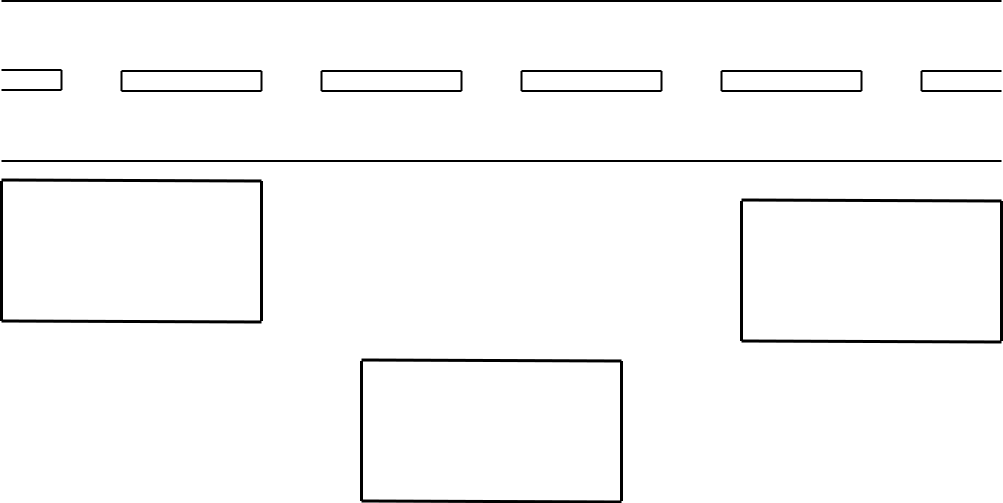
\includegraphics[scale=0.35]{images_ecu/parking_lot.png}
\caption{Parking lot bounded by three cars}
\label{parking_lot}
\end{figure}
\section{Concept of the Algorithm}
The autonomous parking algortihm presented by us is entirely based on the description of motion generation and control for parking an autonomous vehicle in \cite{mgcpav}. The algorithm in the paper consists of three steps: 
\begin{enumerate}
	\item Localization of a parking bay
	\item Adjustment of the vehicle postion to a starting location
	\item Execution of an iterative parking maneuver
\end{enumerate}
Steps one and two are not discussed in detail. The third step is described as iterative task which comprises four steps:
\begin{enumerate}
	\item Obtaining longitudinal and lateral displacement by processing range data
	\item Calculate maneuver duration T and maximum steering angle $\phi_{max}$
	\item Steer the car into the parking bay by controling its velocity and steering angle
	\item Check if parking postion is reached and start with step 1 if not
\end{enumerate}
During all four steps the range data from the sensors is processed. The goal of the algorithm is to control the car only by influencing its velocity and steering angle. It is not desired that the car precisely follows a pre-calculated path.\\
For our purposes we modified the algorithm in two ways and thereby simplified it to a non-iterative 3-phase algorithm. We combined step one and two into one phase called searching phase in which the algorithm finds a parking lot and assumes the car to be positioned correctly for the following maneuver as soon as the lot is found. The third step of the algorithm is split up into two phases. The calculation of the parking parameters T and $\phi_{max}$ takes place in the calculation phase. Performing the actual parking maneuver is done in the controlling phase. Phase 2 and 3 are only carried out once. Therefore our algorithm is no longer iterative.
\subsection{Motion of a vehicle}
In order to be able to move a car using an algortihm one needs to have knowledge about how to mathematically describe its motion. 
Maneuvering a car into a parking lot is a two-dimensional problem. Therefore the car has three degrees of freedom: two coordinates, x and y, and an orientation angle $\theta$. For the algorithm the coordinates refer to the middle of the rear wheel axle. With the help of these the motion can be described by the following equations:
\begin{itemize}
	\item $\dot{x} = v \cdot cos(\phi) \cdot cos(\theta)$
	\item $\dot{y} = v \cdot cos(\phi) \cdot sin(\theta)$
	\item $\dot{\theta} = \frac{v}{L} \cdot sin(\phi)$
\end{itemize}
The change of the coordinate is dependant on the velocity v and the steering angle [phi]. Both of those can be described by formulas which are dependant on a timstamp $t$:
\begin{itemize}
	\item $\phi(t) = \phi_{max} \cdot k_{\phi} \cdot A(t)$ - $k_{\phi}$ indicates the direction of the steering
	\item $v(t) = v_{max} \cdot k_{v} \cdot B(t)$ - $k_{v}$ indicates algebraic sign of the velocity
\end{itemize}
They are used by the algorithm to claculate the actuator data during the parking maneuver. Besides the time dependancy, the forumulas rely on T and $\phi_{max}$. These parameters are calculated within the calculation phase. Both formulas also use the following equations to calculate the ratio of velocity/steering at the timestamp t:
\begin{itemize}
	\item $A(t) = \begin{cases}
					1, \hspace*{3,2cm} 0 \leq t < t'\\
					cos(\frac{\pi(t-t')}{T^*}), \hspace*{1,5cm} t' \leq t \leq T-t'\\
					-1, \hspace*{2,9cm} T-t' < t \leq T\\
				  \end{cases}$
	\item $B(t) = 0.5 \cdot (1 - cos(\frac{4\pi t}{T})), \hspace*{0,6cm} 0 \leq t \leq T$ 
\end{itemize}
where $t' = \frac{T-T^*}{2}$. Using all these equations the motion of a car in a two-dimensional environment can be described.
\subsection{Searching phase} \label{seraching_phase}
In the beginning of the parking procedure the control over the car is handed to the algorithm. The algorithm starts with its first phase: the searching phase. Its goal is to find a suitable parking lot.\\
For our algorithm a suitable parking lot has two main characteristics. On the one hand it offers enough space to park and on the other hand it is bounded by two cars, one in front and one in the back. Empty spaces which are not between two cars or are too small will not be considered. The measurements which qualify a parking bay as suitable are dependant on the measurements of the car as well as predefined safety distances. An adequate parking lot therefore has a minimum length $l_{min}$ and a minimum width $w_{min}$. In order to find such a parking lot the algorithm makes the car move along the traffic lane with constant, slow  speed.  While the controlled car passes parallel parked cars, the algorithm monitors the range data received from the right sensor looking for a potential parking lot. A potential parking lot starts if the range data implies that there is at least $w_{min}$ empty space. As long as this condition is satisfied the algorithm sums up the distance the car traveled since the start of the parking lot. As soon as the range data returns to a value smaller than $w_{min}$ the algortihm checks wether the sumed up distance is as least $l_{min}$ or not. If the parking lot was long enough the algorithm stops the car and transitions into the next phase. If the potential parking lot was too short its length is discarded and the searching phase continues.
\subsection{Calculation phase} \label{calculating}
After the algrotihm successfully finished the searching phase, i.e. a parking bay was found, it continues with the calculation phase. The tasks of the whole phase are carried out while the car is standing still. The purpose of the calculation step is to determine two important parameters for the parking maneuver: the duration T and the maximum steering angle $\phi_{max}$. Both calculations are based on estimations which are then optimized. The duration of the parking maneuver is lower bounded by $T^*$ the time it takes the car to steer from the negative maximum steer angle to the postive maximum steer angle. Therefore we use $T^*$ as an estimation for T. The first estimation for $\phi_{max}$ is the maximum steering angle the controlled car offers. The optimzation of both values relies on the evaluation of the equations for $\dot{x}$, $\dot{y}$ and $\dot{\theta}$ with the helpt of $\phi(t)$ and $v(t)$. The evaluation returns the coordinates of the final postion of the car. On top of that the calculation phase needs a longitudinal condition $C_{long}$ and a lateral condition $C_{lat}$ which indicate wheter the car can still move backwards ($C_{long}$) or to the right ($C_{lat})$. The optimization for T then works as follows:
\begin{enumerate}
	\item Evaluation of equations using T as duration to get end position of the car
	\item Check $C_{long}$
	\item If $C_{long}$ still holds increase T by a small amount and start at step 1
	\item If $C_{long}$ is harmed T is set to the last valid value and the optimzation of T is finished
\end{enumerate}
After we found the optimal value for T we search for the optimal value for $\phi_{max}$. Therefore we check $C_{lat}$. If it holds we know that we already have the optimal value. If $C_{lat}$ does not hold we reduce $\phi_{max}$ by a small amount and evaluate our euqations again before checking $C_{lat}$ again with the new end postion. If $C_{lat}$ is still not fullfilled we iteratively keep reducing $\phi_{max}$ until its optimal value is found. The reduction of $\phi_{max}$ decreases the slope of the car's steering curve which increases the distance of the car to the obstacle to its right after the parking maneuver.
\subsection{Controlling phase}
With all necessary parameters calculated, the algorithm is able to transition into the controlling phase. During this phase the actual parking maneuver is performed. Utilizing the formulas for velocity and steering the algortihm calculates the actuator data for the next simulation step and hands it to the simulation.  For these calculations the optimized parameters from the calculation phase are used. While maneuvering the car, the algorithm always monitors all sensor data in order to prevent crashes. As soon as an upcoming collision is detected the algorithm triggers an emergency stop. After the car is steered into the parking bay the algorithm drives the car backwards until a safety distance contraint is violated. At this point the car is in the parking postion and gets stopped by the algorithm which finished its execution by then.
\section{Implementation}
The implementation of the algorithm is based on three C++ classes/structs. While the \textit{Parking} class implements the actual algorithm, \textit{CarInformation} and \textit{Map} serve as helper classes storing important information which are needed for the algorithm's calculations.
\subsection{CarInformation}
CarInformation is implemented as struct. Its purpose is being a container for car specific data which characterizes the car. As the parking algorithm is working for cars of any sizes CarInformation structs need to be constructed specifically for each car which should be controlled by the algorithm. This happens in the beginning of a Parking scenario. The CarInformation is filled with data by subscribing to the S/A VM which provides necessary information. It contains the following data:
\begin{itemize}
	\item length and width of the car
	\item wheel radius
	\item safety distances (as they depend on car measurements)
	\item max. velocity of the car during the whole parking scenario
	\item max. steering angle the car offers
	\item min. measurements of a suitable parking lot
\end{itemize}
\subsection{Map}
The Map class stores information about the parking lot and the car's starting postion for the parking maneuver. When calling the constructor of a Parking object an empty Map is created. During the process of finding a parking lot the parking lot's measurements and the position of the car are calculated and put into it. The information in a Map plays an important role in the calculation of T and $\phi_{max}$ which is described in \ref{calculating} conceptionally  and in \ref{parking} from the implementaion's point of view.\\
A Map object contains the following information:
\begin{itemize}
	\item coordinates (middle of rear axle) and orientation angle of the car at the beginning of the park maneuver
	\item longitudinal and lateral displacements (length and width of parking lot)
\end{itemize}
Additionally, Map is equipped with getter/setter-methods in oder to access and modify the data.
\subsection{Parking} \label{parking}
The Parking class implements the algorithm. On code-level the algorihtm has four different states:
\begin{itemize}
	\item Searching
	\item Calculating
	\item Controlling
	\item Parked
\end{itemize}
Each of the first three states represents one conecptional phase of the algorithm. The fourth state is entered if the car is in its final parking postion or if an emergency stop is performed. A Parking object maintains a state variable which indicates the current state of the algorithm. The main method of Parking is \textit{receiveData}. It is the only public method and needs six parameters which are all received from the simulation:
\begin{itemize}
	\item sensor\_front - range data from sensor in the front
	\item sensor\_right - range data from sensor to the right
	\item sensor\_back - range data from sensor in the back
	\item spin\_velocity - spin velocity of the car's wheels
	\item timestamp - duration of the current simulation step 
	\item publisher - pointer to the publisher object ehich is called to send acutator data
\end{itemize}
Each time \textit{receiveData} is called the method starts by checking the range data for an upcoming collision which would trigger an emergency stop. Afterwards actuator data for the velocity and the steering angle is calculated and then published. How the actuator data is determined and which values it has depends on the state:\\
\\
\underline{Searching}\\
The initial state of a Parking object is the Searching state. In this state the value of the actuator data is determined based on the return value of the helper function \textit{\_findParkingLot}. The values of \textit{sensor\_right} and \textit{spin\_velocity} are handed to this method as parameters. It uses them to determine whether a suitable parking lot was found or not. If \textit{\_findParkingLot} returns true the car passed a parking lot of reasonable size and all actuator data is set to zero which means the car needs to stop. The algorithm then transitions into the Calculating state. If \textit{\_findParkingLot} return false the velocity actuator value is set to the maximum speed value from the CarInformation struct. In this case the car keeps moving with constant speed as the algorithm keeps searching a parking bay. In order to determine its return value \textit{\_findParkingLot} uses the data of the right sensor and the spin velocity to find a parking lot according to the procdedure described in \ref{seraching_phase}. The total traveled distance is calculated by summing up the traveled distances in each simulation step. The distance covered in the current simulation step can be determined by multiplying the spin velocity with the current timestamp and the wheel radius from CarInformation. Additionally the Map object gets updated.\\
\\
\underline{Calculating}\\
When \textit{receiveData} is called while the algorihtm is in Calculating state the optimzed values of T and $\phi_{max}$ are calculated according to \ref{calculating}. When the constructor of Parking was called both of them were set to their first estimation value. The final value of T is determined by calling the \textit{\_calculate\_T()} method. Within this method the motion equations of the car are evaluated using discrete integration. This procedure is depicted in listing \ref{lst:discrete_integration}. In order to have current values of the velocity and the steering angle the algorithm evaluates \textit{\_velocity} and \textit{\_steering\_angle} in each step of the integration.
\begin{listing}[H]
\begin{minted}[fontsize=\tiny]{c++}
for(double ts = 0; ts <= _T; ts += _sampling_period){
	s_angle = _steering_angle(ts);
    velo = _velocity(ts);

    if(s_angle == 0){
		_phi_old = _phi;
		_phi = _phi;
		_x = _x + (velo * _sampling_period * cos(s_angle));
		_y = _y + (velo * _sampling_period * sin(s_angle));
	} else {
		_phi_old = _phi;
		_phi = _phi + (((velo * _sampling_period) / _info.length_car) * sin(s_angle));
		_x = _x + ((_info.length_car / tan(s_angle)) * (sin(_phi) - sin(_phi_old)));
		_y = _y - ((_info.length_car / tan(s_angle)) * (cos(_phi) - cos(_phi_old)));;
	}
}
\end{minted}
\caption{Discrete integration performed in \textit{\_calculate\_T()} and \textit{\_calculate\_local\_max\_steer()} - Parking.cc (101-116 and 145-160); comments removed}
\label{lst:discrete_integration}
\end{listing}
The evaluation returns the coordinates of the end position of the car. These coordinates are given to the \textit{\_longitudinal\_condition} method which checks the $C_{long}$ condition. If it is fullfilled T is increased by the value of \textit{\_sampling\_period} (value of current timestamp) and another discrete integration is performed. This procedure continues iteratively until $C_{long}$ is no longer satisfied. At this point the last valid value is assigned to T. After T was determined \textit{\_calculate\_local\_max\_steer() is called}. This method checks wether $C_{lat}$ is satisfied. If not $\phi_{max}$ is reduced and the discrete integration is performed again. This is repeated iteratively until $C_{lat}$ is fullfilled and therefore a valid value for $\phi_{max}$ was found. After finishing all calculations the algorithm immediately transitions into the Controlling state.\\
\\
\underline{Controlling}\\
While in Controlling state the actuator data is determined by simply evaluating \textit{\_sterring\_angle} and \textit{\_velocity} with an own timestamp value \textit{\_maneuver\_timestamp}. This value is needed as the parking maneuver needs to start at timestamp 0. After claculating actuator values \textit{\_maneuver\_timestamp} is increased by the current timestamp.\\
\\
\underline{Parked}\\
The Parked state is entered in one of two cases: either the car needed to perform an emergency stop or it reached the parking postion. Regardless of which is the case this state was transitioned to as some range data indicated an collision in the near future. If parked is the current state \textit{receiveData} keeps publishing 0 as actuator data for both, the velocity and the steering angle as the car needs to stand still.
\section{Problems}
Although the algorithm is able to perform all three phases of the algorithm without any disturbances in most of its executions there are still some issues which need to be fixed in order to make it work deterministically for any parking scenario.
\subsection{Safety distances} \label{distances}
During the process of controlling the vehicle's motion the algorithm has some problems in the interplay with SD2. As SD2 is not capable of explicitly setting the velocity of a car, it instead accelerates and brakes in order to reach the velocity which was transmitted as actuator data. Furthermore the controlled SD2-car tends to slide when the algorithm brakes it even at low speed. These issues cause that the car is not stopped instantly if zero is sent as velocity value. As a result of this, crashes occur in the simulation if reasonable safety distances are chosen. Therefore these safety ranges (especially the one in the back of the car) need to be set bigger than necessary. This enlargement has two consequences: the size of suitable parking lots grows considerably and unneeded emergency stops occasionally happen. While larger parking lots are not too much of a problem in a simulation environment, the second problem is more severe. The algorithm stops the car as soon as some sensor's data implies an upcoming collision. With overly large safety distances this behaviour leads to unwanted situations where the algorihtm unnecessarily stops the car. The worst case of this phenomenon occurs during the parking maneuver while the car is being steered into the parking lot as seen in figure \ref{false_emergency}. At this point of time the parking maneuver fails for no actual reason as there is enough space to perform the rest of the maneuver.
\begin{figure}[H]
\centering
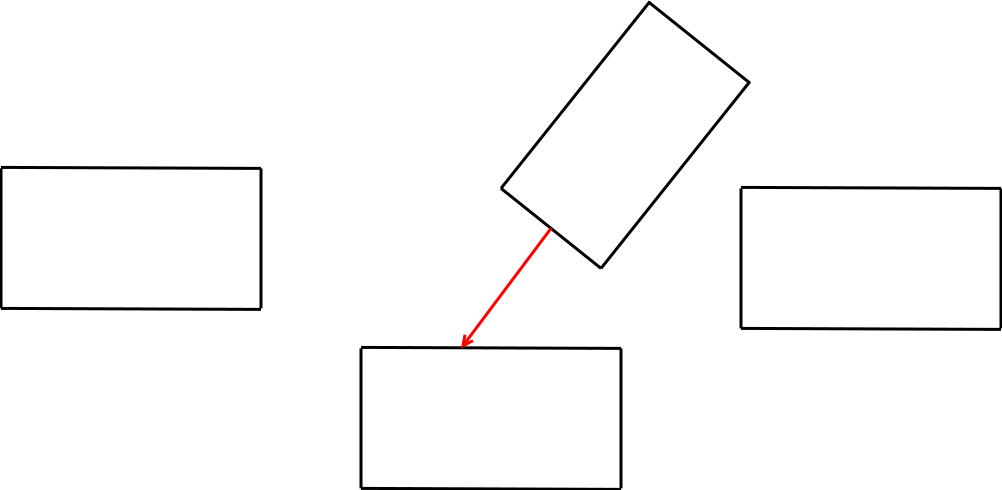
\includegraphics[scale=0.35]{images_ecu/emergency_stop.png}
\caption{Emergency stop due to unnecessary large safety distances}
\label{false_emergency}
\end{figure}
\subsection{Dependance on unrealistic time estimations} \label{dependance}
In the current state of the implementation, the algorithm seems to calculate wrong values for the duration of the parking maneuver T. The problem is that in the calculation phase where T is optimized, only one optimization step is done. This is shown by some sample data in table \ref{table:TandTstar}.
\begin{center}
\label{table:TandTstar}
  \begin{tabular}{  l | r }
    T* & T (optimized) \\
    \hline
    \hline
    5 & 5,0022 \\
    \hline
    10 & 10,0023 \\
    \hline
  \end{tabular}
\end{center}
Conceptionally the number of optimization steps should only depend on the length of the parking lot (longitudinal displacement) as well as the maximum velocity and the maximum steering angle of the car. This means that for any value chosen for T* the optimization should return the same value for T as long as the initial estimation for T* is below the optimized value. Unfortunately this is not the case. As shown by the sample data T* = 5 gets optimized to 5,0022 although it should at least be optimzed to 10,0023.\\
The consequence is that a successful execution of the parking maneuver is entirely reliable on an unrealistic estimation of T* (in our case: 12). The closer the value for T* is chosen to a reasonable value for T which should be calculated automatically, the better the algorithm performs.
\section{Improvements}
\subsection{Rework of calculation phase} \label{rework}
As the value for T do not seem to be calculated correctly as described in \ref{dependance} a possible improvement of the algorithm would be a rework of the calculation phase. In order to do that one would at first need to test the current implementation extensively to find out what the exact problem is. We suspect the calculation of the longitudinal and the lateral conditions to not work as they are intended although it might also be that our implementation of the discrete integration might be buggy.
\subsection{Expanding the parked condition}
The current implementation of the algorithm determines whether the car is parked or not solely on range data received from the sensors. After the algorithm steered the car into the parking bay, the car is forced to drive backwards until a safety distance is violated. This causes the algorihtm to stop the car and go into the PARKED state.
Because of the problem discussed in chapter \ref{distances} this behaviour is justifiable. We need to have overly large parking lots and it therefore makes sense to exceed T in order to drive backwards until a reasonable distance to the obstacle in the back is reached.
Nevertheless it could be necessary to modify this approach. Even though the processing of sensor data will always be necessary in order to support emergency stops this mechanism does not have to be the only way to stop the car after the parking maneuver is finished. The algorithm could be altered in order to stop the car after the time bound T for the parking maneuver is reached. 
Unless the calculation phase is fixed as described in \ref{rework} this modification can possibly lead to scenarios where the car parks fairly far away from the car behind of it.
\subsection{Implementing the original algorihtm}
As we decided to simplify the original algorithm by reducing the interative step to only one step there is the possiblity to expand our algorithm to an iterative algorithm. Such an modification would mean that our calculation and control phases are performed within each iterative step and are therefore performed multiple times. This might increase the precision of the algorithm regarding the positioning of the car. With multiple maneuvering iterations the car is more likely to end up at the optimal parking position. Additionally an algorithm supporting iterative steps should be able to park the car in smaller parking lots. 
\section{Conclusion}
Based on \cite{mgcpav} we implemented an algorithm that is capable of finding a parking lot and perform a parking maneuver autonomously. Due to issues caused by the interplay with SD2 and the calculation of  parking parameters the algorithm does not perform deterministically. Although it parks the car correctly most of the time the algorithm still needs some more optimization. In order to motivate the reader of our paper to do such an optimization, we offered multiple suggestions for improvements.
\bibliography{final-report_group3}

\end{document}
